
\def\theTopic{Interval Estimate }
\def\dayNum{6}

\begin{center}
\vspace*{-.2in}
{\bf {\large Interval Estimate for a Proportion}}\\
\end{center}


If we call someone a ``rat'', we don't mean that they are nice to be
around, but rats might not deserve their bad reputation. Researchers
examining rat's capacity for empathy designed a study in which a pair
of rats were placed in the same cage.  One was trapped in a cramped
inner cage, while the other could move around much more, and could
also free the trapped rat if it chose to do so.  Of thirty pairs of
rats in the experiment, 23 of the free rats released the trapped
rat even though they then had to share the available food.

\begin{center}
  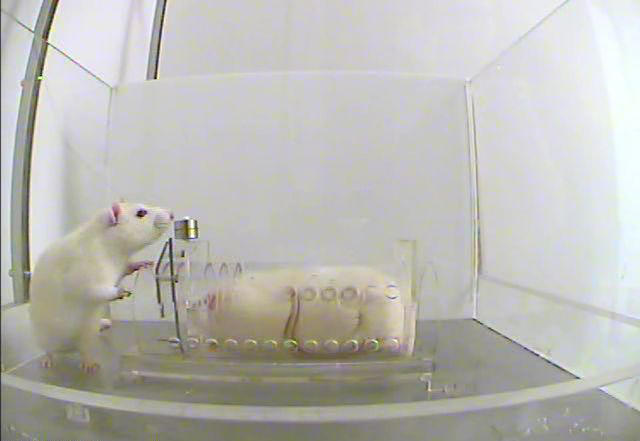
\includegraphics[width=.4\linewidth]{plots/trappedRat.png}
\end{center}

The lab rats  used in the study are genetically identical to other
rats of the same strain, and can be assumed to be a ``representative
sample'' from the population of all rats of this strain.  Researchers
need a good estimate of the true proportion of these rats who would
free another rat trapped in the inner cage.

{\sf Step 1. State the research question.}\vspace{-.1in}
\begin{enumerate}
  \item Based on the description of the study, state the researcher's
   need as a question. 
\begin{students}
  \vspace{1cm}
\end{students}

\begin{key}
{\it How large is the proportion of rats of this strain who show
  ``compassion'' to a trapped rat?}
\end{key}

\end{enumerate}


{\sf Step 2. Design a study and collect data.}\vspace{-.1in}
\begin{enumerate}
  \setcounter{enumi}{1}
  \item \label{RatOptions} What actions of the free rat will be recorded? 
\begin{students}
  \vspace{1cm}
\end{students}

\begin{key}
{\it Free the trapped rat or leave it caged.}
\end{key}

  \item Your answer above gives the outcomes of the  variable of interest in the study.  Is this variable quantitative or categorical?
\begin{students}
  \vspace{1cm}
\end{students}

\begin{key}
{\it  categorical}
\end{key}

  \item  What is the parameter the researchers were interested in?
    Describe it in words and use proper notation to denote it. 
\begin{students}
  \vspace{1cm}
\end{students}

\begin{key}
{\it  $p$, the true proportion of rats of this strain who will free
  a fellow trapped rat.}
\end{key}
\end{enumerate}


{\sf Step 3. Explore and summarize the data.}\vspace{-.1in}
\begin{enumerate}
  \setcounter{enumi}{4}
  \item What is the sample size in this study?  $n = $
\begin{students}
  \vspace{1cm}
\end{students}
\begin{key}
{\it  30}
\end{key}

  \item \label{p.hat} Determine the observed statistic and use correct
    notation to  denote it.
\begin{students}
  \vspace{1cm}
\end{students}

\begin{key}
{\it  $\widehat{p} = 23/30 = 0.7667$}
\end{key}

  \item If the experiment were repeated with another 30 pairs of rats,
    do you think you would get exactly 23 who opened the cage again?
    Explain. 
\begin{students}
  \vspace{2.5cm}
\end{students}

\begin{key}
{\it  Not exactly, A few more or less than 23 would free the trapped
  rat. }
\end{key}
\end{enumerate}



{\sf Step 4. Draw inferences beyond the data. }\\

  The last point is simple, but really important. When we repeat the
  same experiment, we do not get exactly the same results.   Why is
  that?  (Yes, you need to write an answer right here!  The future of
  the world -- no, I mean your success in this course -- depends on it.) 
\begin{students}
  \vspace{2.5cm}
\end{students}

\begin{key}
{\it  Rats differ from each other. We've seen that not all 30 rats
  make the same choice, so if we randomly grab another 30 rats, we
  expect either fewer or more to release the captives, not always 23. }
\end{key}


  We know exactly what proportion of rats in the sample showed
  empathy, and that number makes a good estimate of the same
  proportion of empathetic rats in the population.  However, the fact
  that not all rats, and not all samples are the same tells us we need
  to expect some variation in our sample proportion when we repeat the
  experiment. 

  A single number like the one you computed in
  \ref{p.hat} does not tell the whole story.  We want to let our
  reader know ``how good'' this estimate is.  One way to report the
  quality of an estimate is to give a range of values -- an interval
  estimate --  instead of a  single ``point estimate''.  

  Because we now have easy access to computers, we can run a {\bf
    simulation} to see how variable the statistic might be.  We only
  get one sample of real data, but we can create lots of simulated
  datasets which represent other values which might have been observed.

  
\begin{enumerate}
  \setcounter{enumi}{7}
\item \label{cards} Your group will get 30 cards on which you will write the
  observed outcomes from (\ref{RatOptions}) -- one for each of the 30
  pairs. We don't care about order, just that we get the right
  numbers of cards for each outcome.  Next we simulate another experiment on
  another sample of 30 rat pairs.  We can't actually get more rats and
  study them, so we ``recycle'' the numbers we have.
  \begin{enumerate}
  \item Shuffle your cards and draw one at random. Record the outcome
    for this pair.\\
  \item Replace the card into the deck.  This is a simple but powerful
    idea.  By sampling {\bf with replacement} we have the same
    conditions for every draw, and the probability of each outcome
    stays the same.  Shuffle, draw a card, and record the outcome.
  \item Repeat until you have 30 outcomes chosen at random.  What
    proportion of your rats were freed? \vspace{1cm}
  \end{enumerate}

  The process you just used is called {\bf bootstrapping} (which means
  to make something out of little or nothing), and the 30 outcomes are called a
  bootstrap {\bf resample}.  It's not a sample -- we only get one of
  those -- and we can repeat the resampling process many times.


  \item Reshuffling is slow, so we want to speed up the
    process by using the computer.  Our goal is to see what other
    outcomes we might have gotten for different samples of 30 rat
    pairs. We will again use the \fbox{One Categ.} web app at
    \url{http://shiny.math.montana.edu/jimrc/IntroStatShinyApps/}. 
    Select  ``Enter / Describe Data'' to enter
    the rat data to look like:\\
    \begin{tabular}{lr}
      \fbox{Freed}& \fbox{\  23\  }\\
      \fbox{Not} & \fbox{\  ?? \  }
    \end{tabular}

    Then choose ``Estimate'' from the ``One Categ'' menu.
    What proportion of the rats were freed in your one resample?
\begin{students}
  \vspace{1cm}
\end{students}

\begin{key}
{\it  AWV}
\end{key}

 \item Now resample 100 times and copy the picture you get here.
\begin{students}
  \vspace{4cm}
\end{students}

\begin{key}
  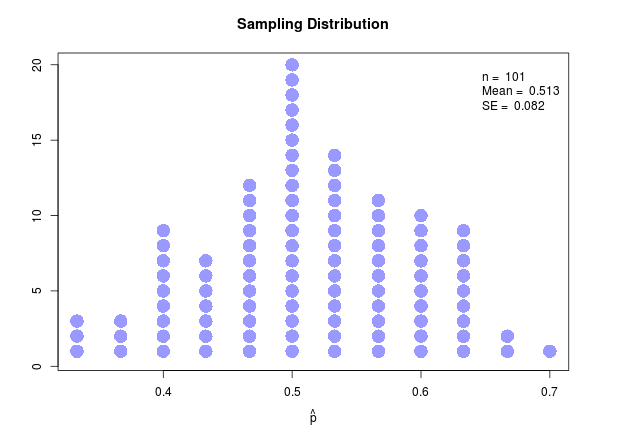
\includegraphics[width=.5\linewidth]{plots/freeRats-101resamples.png}
\end{key} 

   Where is the distribution centered?
\begin{students}
  \vspace{.6cm}
\end{students}

\begin{key}
{\it  approx 0.77}
\end{key}

   How spread out are the sample outcomes? (SE stands for  standard
    error, which is the standard deviation of the resampled values.)
\begin{students}
  \vspace{.6cm}
\end{students}

\begin{key}
{\it  approx 0.078}
\end{key}

 \item The center should seem reasonable.  Why is the distribution
   centered at this value?
\begin{students}
  \vspace{1cm}
\end{students}

\begin{key}
{\it  The simulation is run assuming rats are freed with probability 0.77.}
\end{key}


 \item You should have 101 resampled values in your plot. If not, go
   back to ``Enter/Describe Data'' and change the spelling on the labels (caps
   to lower case, or vice versa). Then come back to ``Estimate'' and
   click \fbox{100} just once.\\
   Below the plot we have options for confidence limits for our
   interval estimate.
   \begin{enumerate}
   \item Click \fbox{80} and count:  How many red points in the left tail?
\begin{key}
{\it  10}
\end{key}
     \\
     How many reds in the right tail?
\begin{key}
{\it  10}
\end{key}
     \\
     How many blue points in the middle?  
\begin{key}
{\it  81}
\end{key}
     \\
   \item Click \fbox{90} and count:  How many red points in the left tail?
\begin{key}
{\it  5}
\end{key}
     \\
     How many reds in the right tail?
\begin{key}
{\it  5}
\end{key}
     \\
     How many blue points in the middle?
\begin{key}
{\it  91}
\end{key}
     \\
  \item Click \fbox{95} and count:  How many red points in the left tail?
\begin{key}
{\it  3}
\end{key}
     \\
     How many reds in the right tail?
\begin{key}
{\it  3}
\end{key}
     \\
     How many blue points in the middle?
\begin{key}
{\it  95}
\end{key}
     \\
   \item Explain how the confidence limit is related to the number of
     blue points.
\begin{students}
  \vspace{1.5cm}
\end{students}

\begin{key}
{\it  With 101 points, the percentage coverage matches the number of
  points left as blue in the middle.}
\end{key}


   \item Play with the ``Confidence Limit'' buttons more to explain:
    How are the endpoints of the interval estimate related to the
    colors of the points in the plot?\begin{students}
  \vspace{1cm}
\end{students}

\begin{key}
{\it} The endpoints are the values at which colors change from red to
blue or vice versa.}
\end{key}

  \item Predict: what will happen to the numbers in each tail for,
    say, a 90 \% interval, if we double the number of resamples?
\begin{students}
  \vspace{1cm}
\end{students}

\begin{key}
{\it  Counts should double, percentages stay the same.}
\end{key}

  \item Click \fbox{100} again and explain: were you right?
\begin{students}
  \vspace{.5cm}
\end{students}
    \end{enumerate}

  \item We need to spend more time on the meaning of ``Confidence'',
    but first let's review:  Explain
   how one dot in the plot was created.  (I suggest going back to how
   you did it manually in \ref{cards}.)
\begin{students}
  \vspace{3cm}
\end{students}

\begin{key}
{\it  We resampled from 30 cards containing 23 ``freed'' and 7 ``not
  freed'' values 30 times.  For each draw, record which type of card
  we get. Compute the proportion of ``freed'' rats in this resample. }
\end{key}
    
 \end{enumerate}


\begin{center}
  {\large \bf Take Home Message} 
\end{center}

Several very BIG ideas:\vspace{-.8cm}
\begin{itemize}
\item We only get one sample, but we can create many ``resamples''
  using sampling with replacement (also called bootstrapping).

\item Interval estimates are better than point estimates.
  \begin{itemize}
  \item They don't pretend to be exact. Any exact value is almost
    certainly wrong.
  \item By looking at the width of an interval we can evaluate the
    quality of the data.  Wide intervals are not very useful.  Skinny
    intervals are more informative.
  \item We can pretend that we know the true value of a parameter in
    order to test our methods.
  \item Our methods are not ``fail safe'', but are actually designed
    to have a certain error rate, for example, 5\% of the time our
    95\% confidence intervals will fail to cover the true parameter.
  \end{itemize}
\item Our confidence in a particular interval is actually in the
  process used to create the interval.  We know that using this
  process over and over again (go out and collect a new random sample
  for each time) gives intervals which will usually
  cover the true value.\\
   We cannot know if a particular interval covered or not, so you have
   to be tolerant of some uncertainty.  We will explore this more in
   your next class period.
 \item 
  Use the remaining space for any questions or your own summary of the
  lesson. 
\end{itemize}



